\chapter{Conception}
\section*{Introduction}
After identifying the functional and non-functional needs and the main functionalities of our application. We begin this part
of the conceptual study by describing the general architecture of our system and
it's detailed internal modeling through class and sequence diagrams.
\section{Global Architecture}
In this section, we will give an overview of the definition of the
the architectural pattern was chosen to model our application and we will
detail the projection of this pattern on our application.

\subsection{Definition of the Model-View-Controller design pattern}
Our chosen architecture of work for this project will be the MVC  architecture since it is recommended by the Salesforce developer’s community.\\
The model-view-controller (MVC) design pattern specifies that an application consists of a data model, presentation information, and control information.\cite{5} \\
The pattern requires that each of these be separated into different objects:
\begin{itemize}
\item \textbf{The model} (for example, the data information) contains only pure application data; it contains no logic describing how to present the data to a user. \cite{5}
\item \textbf{The view} (for example, the presentation information) presents the model's data to the user. The view knows how to access the model's data but does not know what this data means or what the user can do to manipulate it. \cite{5}
\item \textbf{The controller} (for example, the control information) exists between the view and the model. It listens to events triggered by the view (or another external source) and executes the appropriate reaction to these events. In most cases, the reaction is to call a method on the model. Since the view and the model are connected through a notification mechanism, the result of this action is then automatically reflected in the view.\cite{5}
\end{itemize}
Thanks to these principles, the components of the application become easy to
manage, test, modify, and reuse.\\
The following figure explains furthermore the role and the idea behind each component of the MVC pattern:

\begin{figure}[H]%
    \center   
    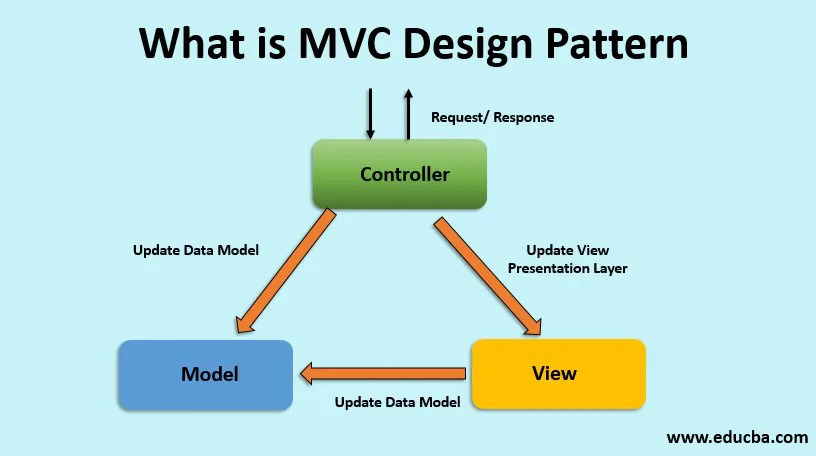
\includegraphics[scale=0.5]{mvc2.jpg}
    \caption{Understanding MVC Design Pattern, Source: \cite{7}}
\end{figure}
\subsection{Application of the "MVC" pattern}
We explain in this paragraph the details of the projection of the pattern
MVC on our app.\\
The following figure represents the class diagram which illustrates the binding
between entities (classes). Indeed, this diagram translates the content of the \textbf{Model} component, and it's based on the schema that is already established within the Salesforce infrastructure.
\begin{figure}[H]%
    \center   
    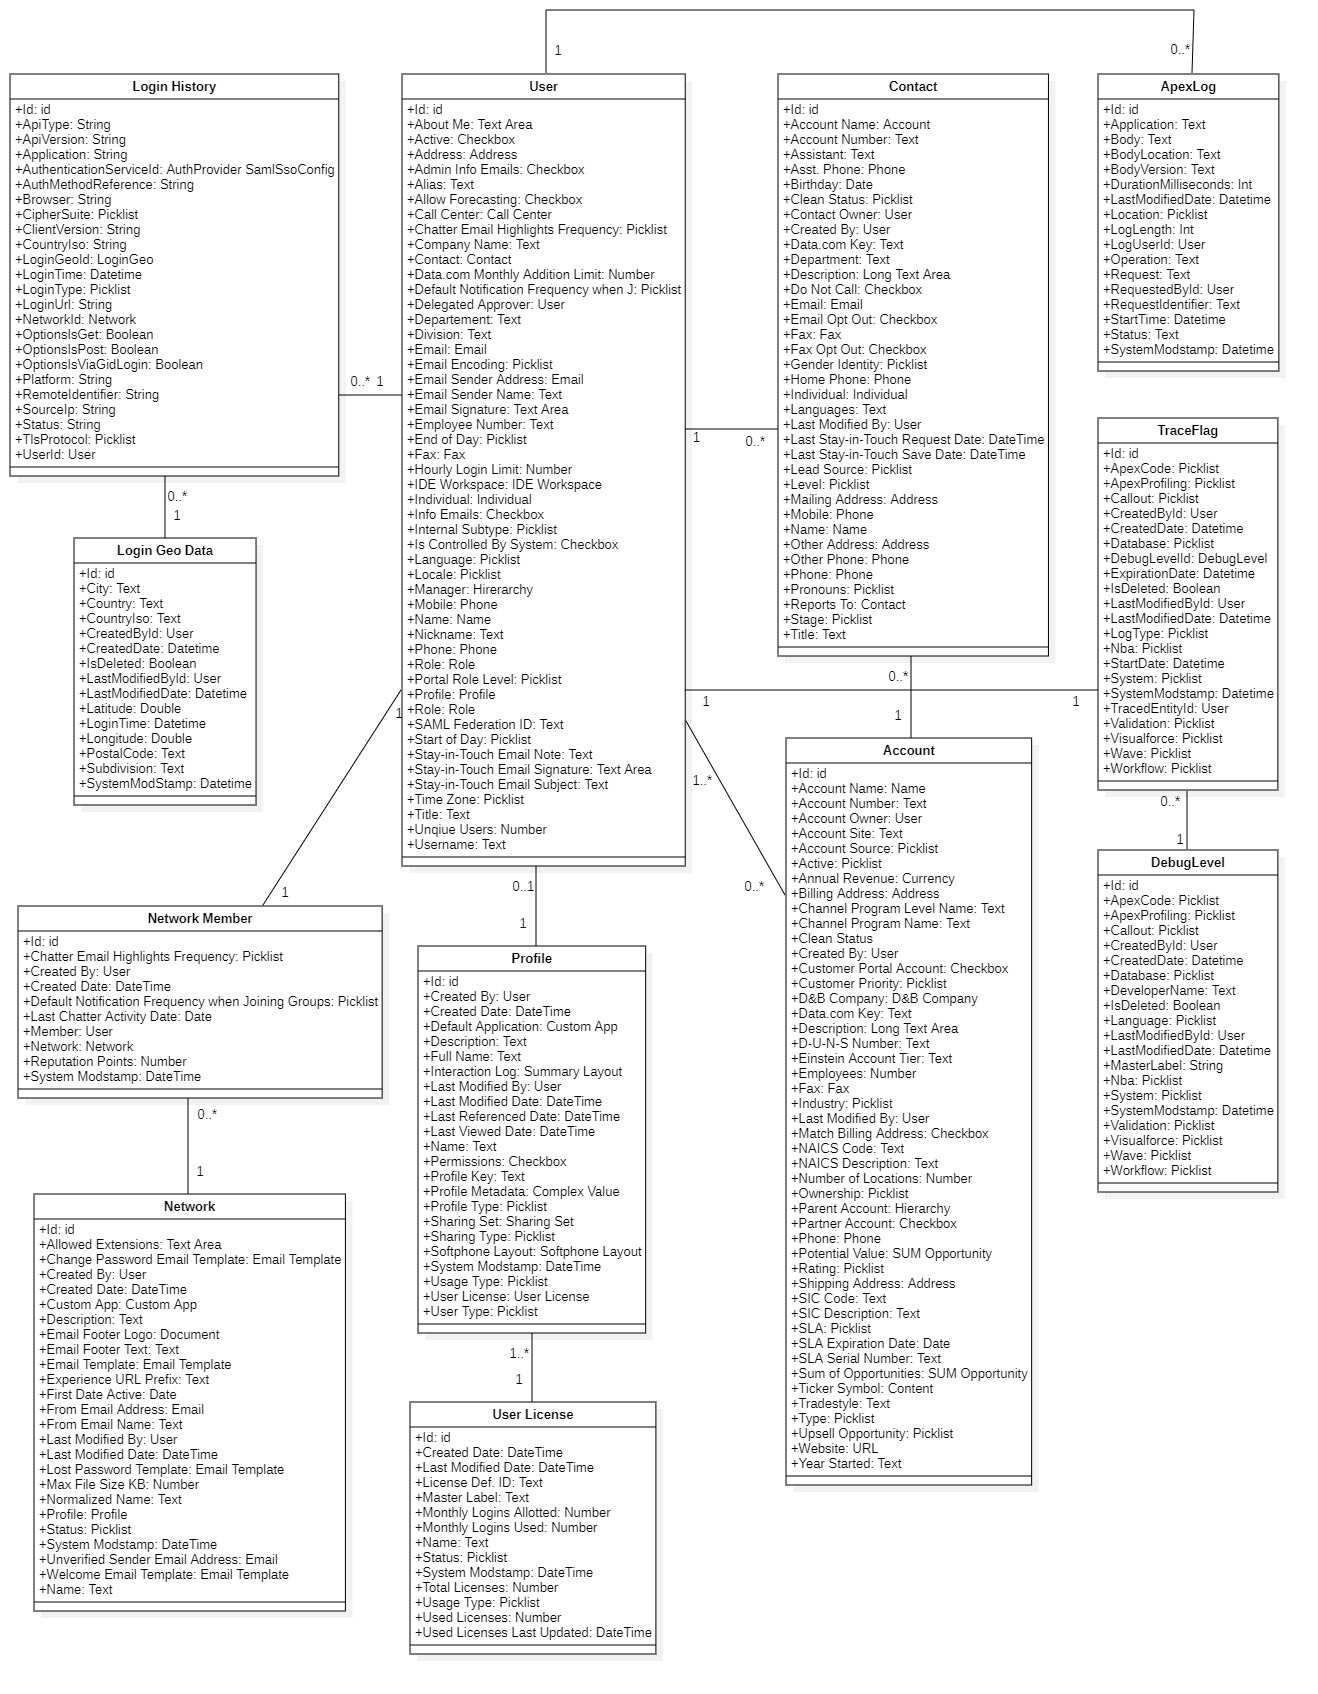
\includegraphics[scale=0.4]{ClassDiagram.jpg}
    \caption{Class diagram representing the "Model" component}
\end{figure}
\newpage
Description of classes representing our Model:
\begin{itemize}
\item \textbf{User:}\\
This class represents our application's Salesforce user who is the main focus of the administrator and the community manager when working within our app. This class's most important attributes in our application are:
\begin{itemize}
\item[•] Id: the unique identification key for the user 
\item[•] Active: determines the status of the user (active or not active)
\item[•] Address: the full address of the user
\item[•] Alias: the alias of the user, usually composed of the first letter of his first name and his last name concatenated together
\item[•] Contact: a lookup field that connects the user to its corresponding Salesforce contact which is necessary to have to allow the user to access a community
\item[•] Email: the email of the user
\item[•] Email Encoding: the encoding of the user's email (for example UTF-8), useful for sending appropriate emails to the user
%\item[•] First Name: the first name of the user
\item[•] Is Portal Enabled: determines if the user can access a community or not
%\item[•] Last Name: the last name of the user
\item[•] Language: the preferred interface language of the user that will control the user interface of the accessed community
\item[•] Locale: the geolocation locale id of the user ( example Arabic(Tunisia) )
\item[•] Name: the full name of the user which is composed automatically by the Salesforce system by concatenating his first name and his last name
\item[•] Profile: a lookup field that connects the user to its corresponding Salesforce profile which controls the level of access provided to the user ( for example System Administrator which gives full access to all Salesforce objects and configurations )
\item[•] Role: the relative company role of the user ( for example CEO ), this field is required to be able to add a user to a community through our app
\item[•] Time Zone: the timezone of the user ( for example GMT+02:00 )
\item[•] Username: the unique Salesforce user name if the user usually identical to the user's email
\end{itemize}
\item \textbf{Contact:}\\
This class represents the Salesforce contacts connected to the community user in our application. This class's most important attributes in our application are:
\begin{itemize}
\item[•] Id: the unique identification key for the contact 
\item[•] Account Name: a lookup field that represents the Salesforce unique account connected to the contact
\item[•] Contact Owner: a lookup field that represents the user owning the Salesforce contact
\item[•] Created By:: a lookup field that represents the user who created the Salesforce contact
\item[•] Email: email of the contact
\item[•] Last Modified By: a lookup field that represents the last user to modify details of the contact
\item[•] Name: the full name of the contact

\end{itemize}
\item \textbf{Account}\\
This class represents the Salesforce account connected to the community user in our application. This class's most important attributes in our application are:
\begin{itemize}
\item[•] Id: the unique identification key for the account 
\item[•] Account Name: Salesforce account name
\item[•] Account Owner: a lookup field that represents the user owning the Salesforce account 
\item[•] Created By: a lookup field that represents the user who created the Salesforce account 
\item[•] Customer Portal Account: determines if the account can be connected to the community user
\item[•] Last Modified By: a lookup field that represents the last user to modify details of the account
\item[•] Parent Account: a self-lookup field that represents the parent account of this account through the Salesforce hierarchy
\end{itemize}
\item \textbf{Profile}\\
This class represents the Salesforce profile connected to the community user in our application. This class's most important attributes in our application are:
\begin{itemize}
\item[•] Id: the unique identification key for the profile 
\item[•] Created By: a lookup field that represents the user who created the Salesforce profile 
\item[•] Full Name: the full name of the profile that represents its usage context 
\item[•] Last Modified By: a lookup field that represents the last user to modify details of the profile
\item[•] Name: the name of the Salesforce profile that represents the main way of identifying the profile through other objects
\item[•] User License: a lookup field that represents the Salesforce purchased user license connected to the profile 

\end{itemize}
\item \textbf{User License}\\
This class represents the Salesforce purchased user license connected to the community user in our application. This class's most important attributes in our application are:
\begin{itemize}
\item[•] Id: the unique identification key for the user license 
\item[•] Name: the name of the Salesforce user license that represents the main way of identifying the user license through other objects
\item[•] Total Licenses: represents the total number of purchased user licenses dedicated to community users 
\item[•] Used Licenses: represents the number of used user licenses which determines if the administrator or the community manager can add more users to his community depending on how many purchased user licenses are left

\end{itemize}
\item \textbf{Network}\\
This class represents the community created by the administrator or the community manager in our application. This class's most important attributes in our application are:
\begin{itemize}
\item[•] Id: the unique identification key for the network 
\item[•] Created By: a lookup field that represents the user who created the Salesforce community 
\item[•] Created Date: represents the date and time of the creation of the Salesforce community
\item[•] Description: a brief description of the community set by its creator to summarize its purpose
\item[•] From Email Address: represents the email that will be displayed when a user receives an email through our application
\item[•] From Email Name: represents the name that will be displayed when a user receives an email through our application
\item[•] Last Modified By: a lookup field that represents the last user to modify details or the content of the community
\item[•] Last Modified Date: represents the date and time of the last activity within the community
\item[•] Lost Password Template: represents the email template that will be used when sending a "Reset password" email through our application
\item[•] Name: the name of the Salesforce community that represents the main way of identifying the community through other objects
\item[•] Profile: a lookup field that represents the Salesforce profiles that are allowed to access the community
\item[•] Welcome Email Template: represents the email template that will be used when sending a "Welcome to community" email through our application
\end{itemize}
\item \textbf{Network Member}\\
This class represents the users that are considered members of a Salesforce community in our application. This class's most important attributes in our application are:
\begin{itemize}
\item[•] Id: the unique identification key for the network member
\item[•] Created By: a lookup field that represents the user who added the new member to the Salesforce community 
\item[•] Member: a lookup field that represents the user representing the member of the community, this field is used to access all the details about the user within the Network Member object
\item[•] Network: a lookup field that represents the community that the member is considered a part of, this field is used to access all the details about the community within the Network Member object


\end{itemize}

\item \textbf{Login History}\\
This class represents the login event details that are recorded by Salesforce regarding users' activity and will be used to track the activities of the members of any Salesforce community in our application. This class's most important attributes in our application are:
\begin{itemize}
\item[•] Id: the unique identification key for the login history
\item[•] Browser: represents the commercial name and the version of the web browser that the login vent happened from ( for example Chrome 112 ) 
\item[•] CountryIso: the first two letters of the country where the login event happened from ( for example TN stands for Tunisia )
\item[•] LoginGeoId: a lookup field that represents the geographic location connected to the login event
\item[•] LoginTime: the exact date and time of the login event
\item[•] NetworkId:  a lookup field that represents the community that the user wanted to access when the login event was recorded
\item[•] Platform: represents the commercial name and the version of the platform that the login vent happened from ( for example Windows 10 )
\item[•] SourceIp: the IP address of the user that tried to access the community 
\item[•] Status: the state of the login attempt ( for example Invalid Password )
\item[•] UserId: a lookup field that represents the user concerned with the login event, this field is used to send security warning emails, within our application, to users concerned with a failed login attempt 

\end{itemize}
\item \textbf{LoginGeo}\\
This class represents the login event's geographic location details that are recorded by Salesforce regarding users' activity and will be used to track the geographic location of the activities of the members of any Salesforce community in our application. This class's most important attributes in our application are:
\begin{itemize}
\item[•] Id: the unique identification key for the loginGeo
\item[•] City: represents the city when the login event happened (for example Mahdia)
\item[•] Country: represents the country when the login event happened (for example Tunisia)
\item[•] CountryIso: the first two letters of the country where the login event happened from ( for example TN stands for Tunisia )
\item[•] Latitude: represents the geographic latitude of the login event
\item[•] Longitude: represents the geographic longitude of the login event

\end{itemize}
\item \textbf{TraceFlag}\\
This class represents the tracked users and entities regarding monitoring logs for programming errors and bugs committed by developers in the community and will be used to register said users so that their error logs will be monitor by the administrator. This class's most important attributes in our application are:
\begin{itemize}
\item[•] Id: the unique identification key for the traceFlag
\item[•] StartDate: represents the tracking event's starting date for the created trace flag
\item[•] ExpirationDate: represents the expiration date for the created trace flag
\item[•] DebugLevelId: a lookup field that connects the traceflag to the Debulevel object in Salesforce , in our application this field will have the default value of the SFDC DevConsole's Id 
\item[•] LogType: determines the type of logging that will be returned when requesting it, in our application it will take the default value of "USER \_ DEBUG" since we will be tracking users error logs
\item[•] TracedEntityId: represents the id of the tracked user

\end{itemize}
\item \textbf{DebugLevel}\\
This class represents a configuration setting that determines the level of detail for debugging and logging activities in the system. This class's most important attributes in our application are:
\begin{itemize}
\item[•] Id: the unique identification key for the debugLevel
\item[•] MasterLabel: represents debugLevel main label that will be used in our application to retrieve the id of the object and connect it to the TraceFlag object

\end{itemize}
\item \textbf{ApexLog}\\
This class represents the detailed logs of the execution of all Apex code ran by the tracked user within the community, and it will be used in our application to provide said logs the administrator. This class's most important attributes in our application are:
\begin{itemize}
\item[•] Id: the unique identification key for the apexLog
\item[•] Body: represents the plain text containing execution traces, debug operations and outputs and errors provided by the called Apex methods
\item[•] LogUserId: a lookup field representing the user who ran the Apex code which generated the ApexLog
\item[•] StartDate: represents date and time marking the beginning of the Apex code's execution
\item[•] Status: represents the title of the main event's log (for example out of bound exception)

\end{itemize}
\end{itemize}
%End of page 35 in the Selma report%
The classes we have defined in the "Entities" layer are related to the German business field, employable in various types of commercial applications, and
independent of our application. Thus, we made the
principle of independence between the business rules and the application rules.\\
For the rest of the layers of the Clean architecture pattern, we will describe
the dependencies between these layers by giving an example of a connection between a
set of classes belonging to these layers.
The following figure represents the general dependence in our case between the
layers of the clean architecture pattern.
\begin{figure}[H]%
    \center   
    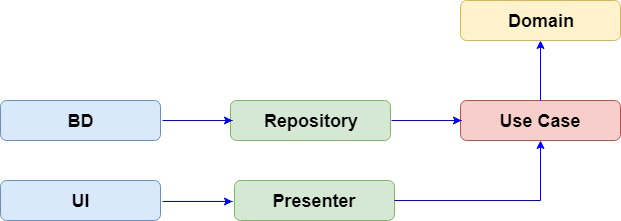
\includegraphics[scale=0.5]{ca_dep.png}
    \caption{General dependency diagram}
\end{figure}
\begin{itemize}
\item The domain layer (Entities) is independent of all layers.
\item The application layer (Usecase) depends on the domain layer and is independent of other layers. This layer prepares responses to
user queries using entities.
\item The adapters interface layer depends on the application(Usecase) layer.
This layer transmits the user request and the necessary data
to its processing at the Use Cases layer and retrieves the response and structure
for the User Interface component.
\item The user interface (UI) component of the "External technologies" layer
depends on the interface layer adapters through the Presenter an n
pass the user's request to it and retrieves the response.
\item The database component of the "External technologies" layer
allows the Use Case layer to retrieve data through a
Gateway(Repository) belonging to the Interface Adapter layer.

\end{itemize}
The following figure shows an example of a detailed dependency between
layers of the clean architecture pattern in the case of our application. These dependencies link a set of classes belonging to the different layers.
These classes realize the example of the functionality of displaying the list of
users.
\begin{figure}[H]%
    \center   
    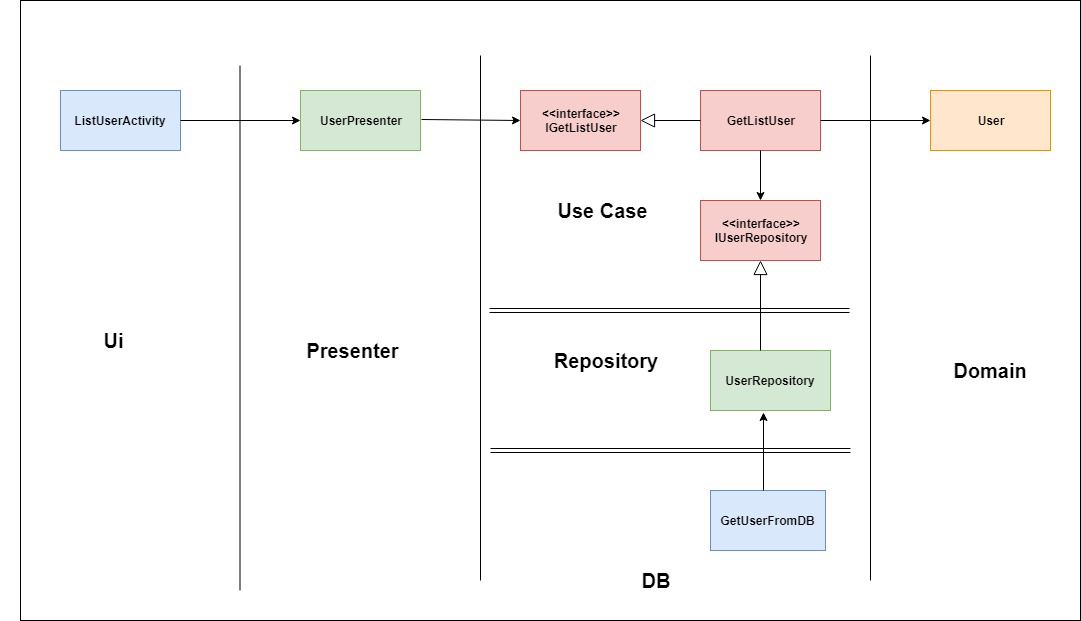
\includegraphics[scale=0.5]{ca_dep_detail.png}
    \caption{Detailed dependency diagram in case of functionality
print the list of users}
\end{figure}
According to the figure, the Interface Adapter layer (UserPresenter and UserRepository)
communicates (passing and retrieving data) with the Use layer
boxes by implementing or instantiating its IGetListUser and IUser-
Repository. These interfaces represent the "ports" of the Use Cases layer.
This example shows how we realized the principle of independence
from the core of the application of the technologies used. No instance of the
adapters interface layer or outer layer exists in the app's core.
\section{Dynamic view of the application}
In this section, we will describe the internal dynamic of our application using sequence diagrams and activity diagrams
\subsection{Detailed sequence diagram of the "register" use case}
The following figure illustrates the detailed sequence diagram of the use case
"Register".
This use case starts with opening a registration interface
for the user. Then, the user enters his coordinates and confirms them.
The system displays an error message if the email already exists otherwise it redirects
the user to the home page. 
\begin{figure}[H]%
    \center   
    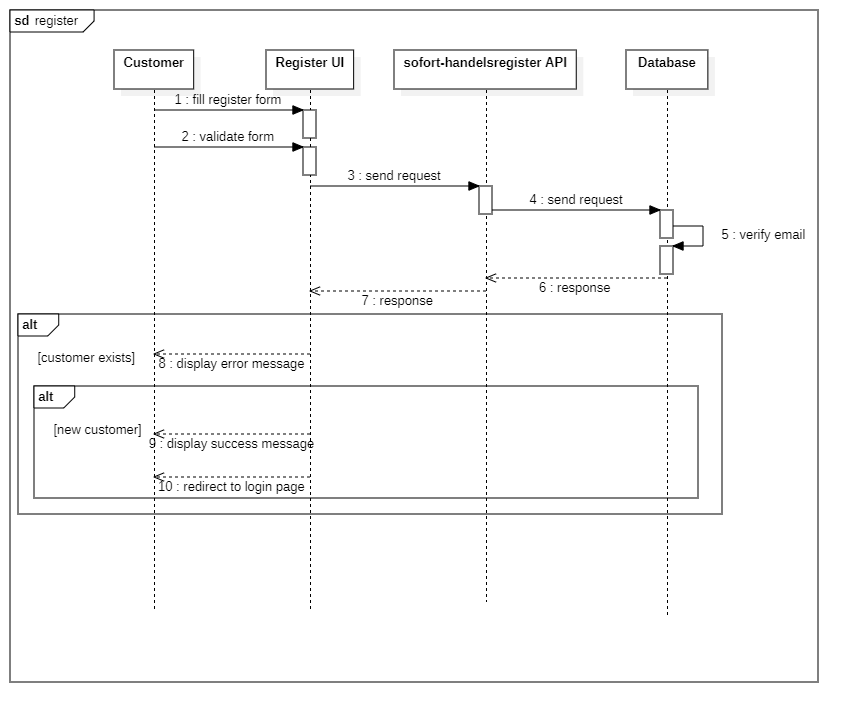
\includegraphics[scale=0.5]{seq_r.png}
    \caption{Detailed sequence diagram of the "register" use case}
\end{figure}
\subsection{Detailed sequence diagram of the "login" use case}
The following figure illustrates the detailed sequence diagram of the use case
"login".
This use case starts with opening a login interface
for the user. Then, the user enters his email and password then confirms them.
The system displays an error message if the email or the password is incorrect otherwise it redirects
the user to the home page.
the user may also choose to log in using a social media account ( Google, Facebook, LinkedIn, Xing), by taping the dedicated button to each social media which will redirect him to the interface provided by that specific social media API, the user will be redirected to the home interface upon successful social media login.
  \begin{figure}[H]%
    \center   
    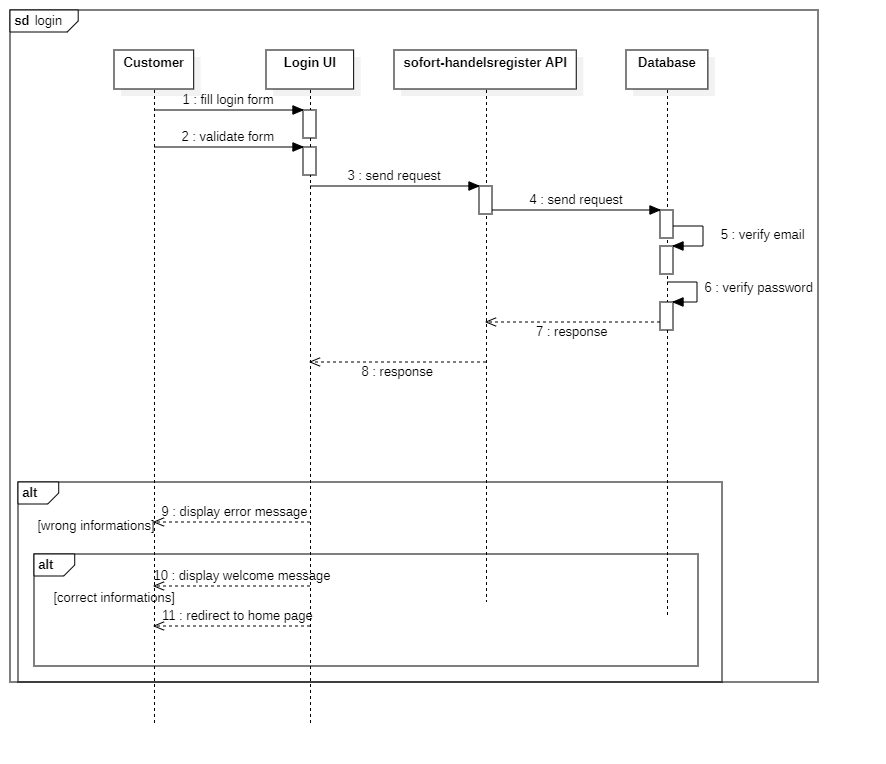
\includegraphics[scale=0.5]{seq_l.png}
    \caption{Detailed sequence diagram of the "login" use case}
\end{figure}
\begin{figure}[H]%
    \center   
    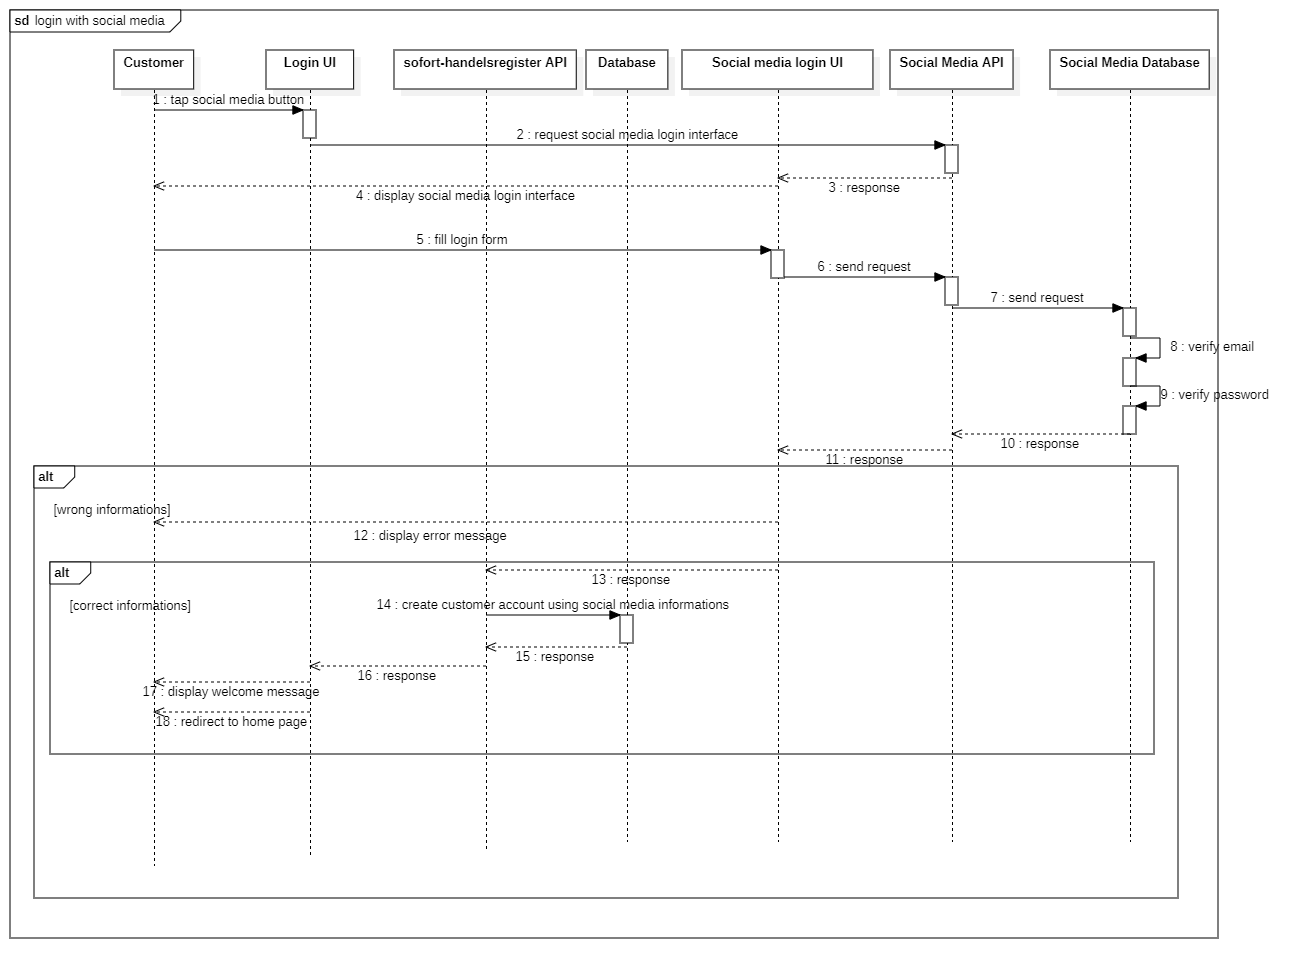
\includegraphics[scale=0.4]{seq_ls.png}
    \caption{Detailed sequence diagram of the "login with social media" use case}
\end{figure}
\subsection{Detailed sequence diagram of the "search company" use case}
The following figure illustrates the detailed sequence diagram of the use case
"search company".
This use case starts with opening an interface for the company's search for the user. Then the user enters the name of the wanted company's name or the first letters of its name, he may also add some filter to the results using a different interface (by state, zip code, legal form, capital, branch), upon confirming his request the interface will prompt an interactive list of results where the user may tap one of them to access more detailed information about it.
 \begin{figure}[H]%
    \center   
    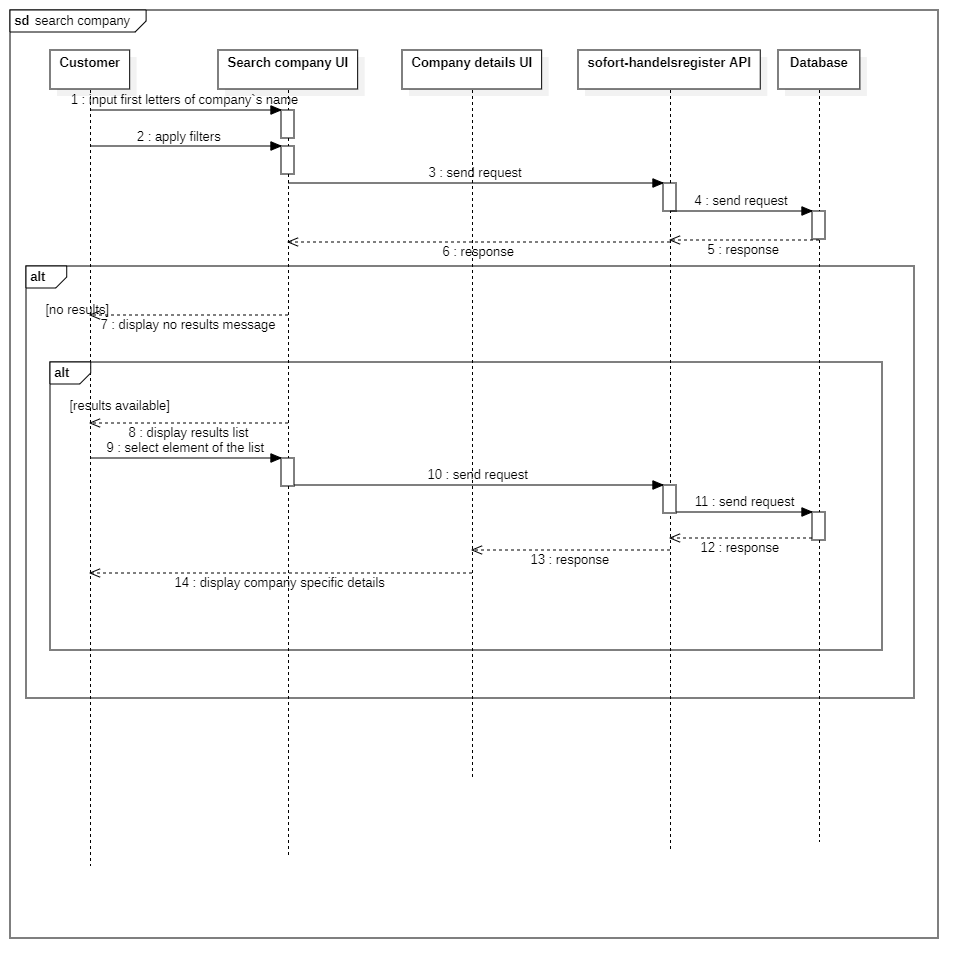
\includegraphics[scale=0.5]{seq_s.png}
    \caption{Detailed sequence diagram of the "search company" use case}
\end{figure}

\subsection{Detailed sequence diagram of the "follow company" use case}
The following figure illustrates the detailed sequence diagram of the use case
"follow company".
This use case starts with opening an interface containing specific company details for the user. Then the user may tap the follow button to add that company to his tracked companies list and start receiving notifications about it, these notifications may be deactivated later in the tracked companies interface.
\begin{figure}[H]%
    \center   
    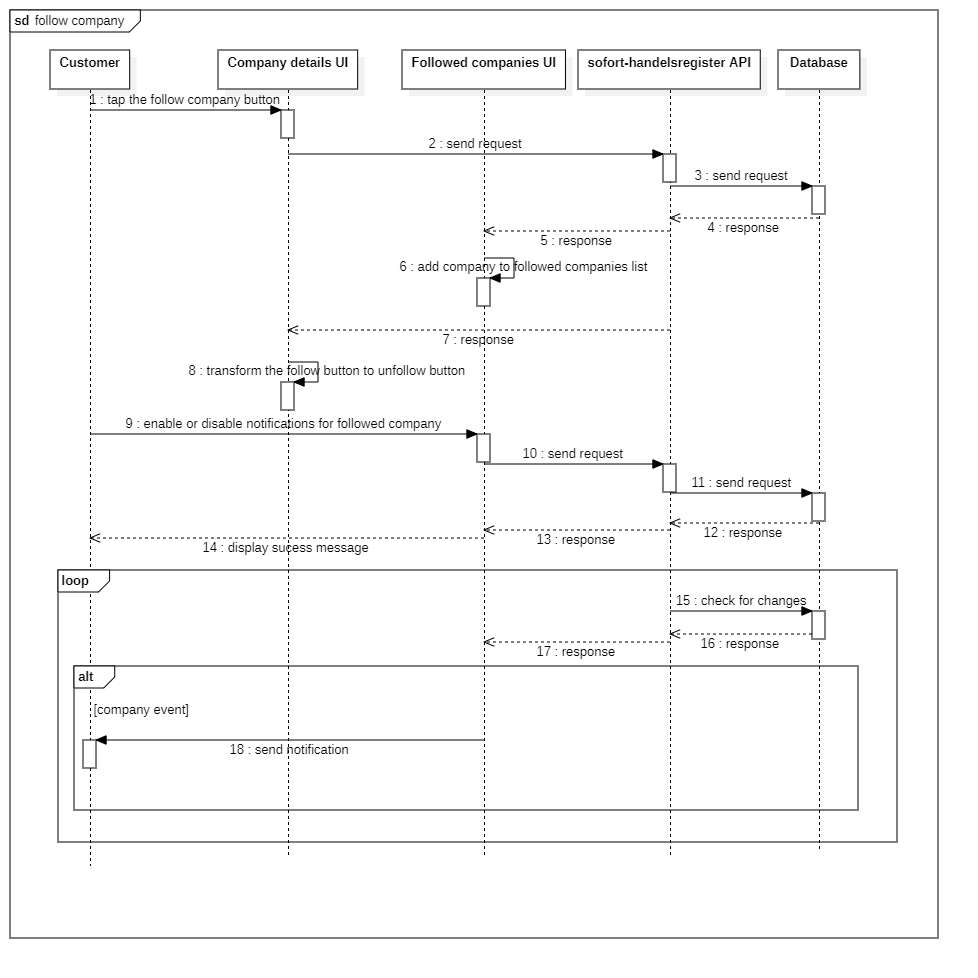
\includegraphics[scale=0.5]{seq_f.png}
    \caption{Detailed sequence diagram of the "follow company" use case}
\end{figure}
\subsection{Detailed sequence diagram of the "purchase documents" use case}
The following figure illustrates the detailed sequence diagram of the use case
"purchase documents".
This use case starts with opening an interface containing specific company details for the user. Then the user may scroll down to the documents section and add wanted documents to his cart, after that he may checkout and finalize his purchase process after filling in his credit card details. As a result, the purchased documents are added to the user's inventory interface and he may download them.
\begin{figure}[H]%
    \center   
    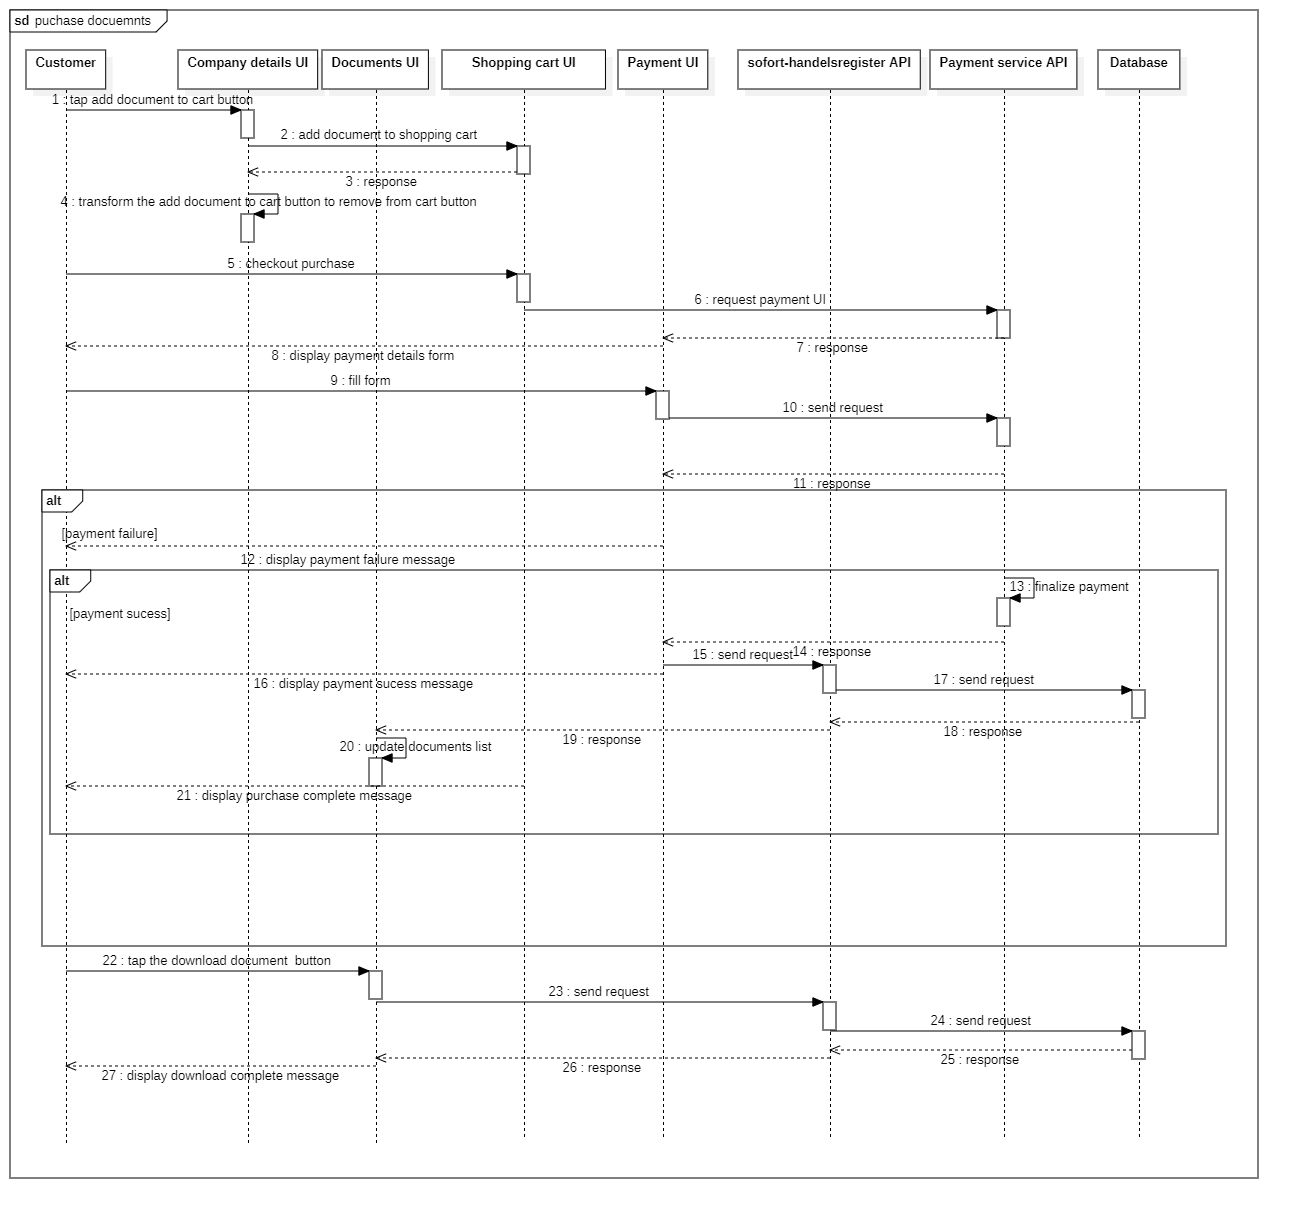
\includegraphics[scale=0.4]{seq_p.png}
    \caption{Detailed sequence diagram of the "purchase documents" use case}
\end{figure}
\section*{Conclusion}
This chapter presents one of the most important phases of the process of
development of a project: design subdivided into the overall design
and detailed design.\\
We presented a Clean Architecture architecture pattern and we
explained its application in our case. We have described the dynamic view
of the system through a set of sequence diagrams and diagrams
of activities.\\
The following chapter will deal with the realization of the project illustrated by screenshots of different interfaces. We will describe the environment of
work and the tools used too.